
%% General definitions
\documentclass{article} %% Determines the general format.
\usepackage{a4wide} %% paper size: A4.
\usepackage[utf8]{inputenc} %% This file is written in UTF-8.
%% Some editors on Windows cannot save files in UTF-8.
%% If there is a problem with special characters not showing up
%% correctly, try switching "utf8" to "latin1" (ISO 8859-1).
\usepackage[T1]{fontenc} %% Format of the resulting PDF file.
\usepackage{fancyhdr} %% Package to create a header on each page.
\usepackage{lastpage} %% Used for "Page X of Y" in the header.
%% For this to work, you have to call pdflatex twice.
\usepackage{enumerate} %% Used to change the style of enumerations (see below).

\usepackage{amssymb} %% Definitions for math symbols.
\usepackage{amsmath} %% Definitions for math symbols.

\usepackage{tikz}  %% Pagacke to create graphics (graphs, automata, etc.)
\usetikzlibrary{automata} %% Tikz library to draw automata
\usetikzlibrary{arrows}   %% Tikz library for nicer arrow heads
\usetikzlibrary{arrows.meta}   %% Tikz library for nicer arrow heads
\usetikzlibrary{positioning}   %% Tikz library for nicer arrow heads


%% Left side of header
\lhead{\course\\\semester\\Exercise \homeworkNumber}
%% Right side of header
\rhead{\authorname\\Page \thepage\ of \pageref{LastPage}}
%% Height of header
\usepackage[headheight=36pt]{geometry}
%% Page style that uses the header
\pagestyle{fancy}

\newcommand{\authorname}{Alex Lutsch\\Ephraim Siegfried }
\newcommand{\semester}{Fall Semester 2023}
\newcommand{\course}{Discrete Mathematics in Computer Science}
\newcommand{\homeworkNumber}{7}


\begin{document}



\section*{Exercise \homeworkNumber.1}

\begin{enumerate}[(a)]
	\item I will disprove the statement with a counter example. For \( a = b = c = 2 \) we have that \( a \mid c \) and \( b \mid c \) is true because we have \( ak = bk = 2k = c = 2 \) for \( k = 1 \). But \( ab \mid c \) which is equivalent to \( 4 \mid 2 \) is not true because there exists no \( k \in \mathbb{Z} \) such that \( abk = 4k = 2 = c\). Therefore \( a \mid c \) and \( b \mid c \) does not imply \( ab \mid c \).
	\item If \( a \mid b \) and \( a \mid b-c \) there exist \( k_{1}, k_{2} \in  \mathbb{Z} \) s.t. \( ak_{1} = b \) and \( ak_{2}=b-c \). By substitution we get \( ak_{2} = ak_{1}-c \leftrightarrow ak_{1} - ak_{2} = c \leftrightarrow a(k_{1}-k_{2}) = c \). We have that \( k_{1}-k_{2} = k_{3} \in \mathbb{Z} \). Therefore \( ak_{3} = c \) which implies \( a \mid c \).
\end{enumerate}



\section*{Exercise \homeworkNumber.2}

\begin{enumerate}[(a)]
	\item
	      Given $a \equiv b $ (mod n) we want to show that $a*k \equiv b*k$ for all $k \in \mathbb Z$.\\
	      As $n \lvert a-b$ there exists a $c \in \mathbb Z$ so that $c*n = a-b$. \\
	      Multiplying both sides with $k \in \mathbb Z$ we get $kcn = k(a-b)$ and thus $kn \lvert k(a-b)$, which shows that $a*k \equiv b*k$.
	\item
	      Given $a \equiv b $ (mod n) we want to show that $a^k \equiv b^k$ for all $k \in \mathbb N_0$. \\
	      As $n \lvert a-b$ there exists a $c \in \mathbb Z$ so that $c*n = a-b$. \\
	      Putting $k \in \mathbb N_0$ as exponent on both sides we get $(cn)^k = (a-b)^k$ and thus $n^k \lvert (a-b)^k$, which shows that $a^k \equiv b^k$.
\end{enumerate}



\section*{Exercise \homeworkNumber.3}

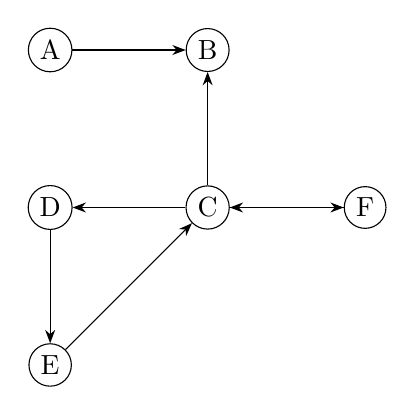
\begin{tikzpicture}[->,>=Stealth,node distance=2cm,on grid,auto]
	\node[circle, draw, inner sep=2pt] (A) {A};
	\node[circle, draw, inner sep=2pt] (B) [right=of A] {B};
	\node[circle, draw, inner sep=2pt] (C) [below=of B] {C};
	\node[circle, draw, inner sep=2pt] (D) [below=of A] {D};
	\node[circle, draw, inner sep=2pt] (E) [below=of D] {E};
	\node[circle, draw, inner sep=2pt] (F) [right=of C] {F};

	\draw (A) to (B);
	\draw (C) to (B);
	\draw (C) to (D);
	\draw (C) to (F);
	\draw (D) to (E);
	\draw (E) to (C);
	\draw (F) to (C);
\end{tikzpicture}


\section*{Exercise \homeworkNumber.4}
The graph \( G = (V,E) \) with \\
\( V = \left\{ H, I, J, K, L, M, N  \right\}  \) and \\
\( E = \left\{ \left\{ K, J \right\}, \left\{ K,M \right\}, \left\{ K,N \right\}, \left\{ K,H \right\}, \left\{ K,L \right\}, \left\{ J,M \right\}, \left\{ M,N \right\}, \left\{ M,L \right\}   \right\} \) \\
satisfies the properties.



\section*{Exercise \homeworkNumber.5}

\begin{enumerate}[(a)]
	\item The walk \( \pi =  \left< D,B,A,B \right> \) from D to B is not a path.
	\item The set \( P = \left\{ \left< A, B, C \right>, \left< C, B, A \right>, \left< D,B,A \right>, \left< D,B,C \right> \right\}   \) contains all paths with length 2.
	\item The tour \( \left< A \right> \) satisfies \( v_{0} = v_{n} = A \) and is not a cycle.
	\item There are 6 cycles in the graph.
\end{enumerate}



\end{document}
